\documentclass[12pt]{report}
\usepackage[utf8]{inputenc}
\usepackage{graphicx}
\usepackage{pgfplots}
\usepackage{float}
\usepackage[italian]{babel}
\pgfplotsset{compat=newest}
\usepackage{amsfonts}
\usepackage{amssymb}
\usepackage{geometry}
\usepackage{amsmath}
\usepackage{amsthm}
\usepackage[hidelinks]{hyperref}
\usepackage{algorithm}
\usepackage{algpseudocode}
\usepackage{marvosym}

\theoremstyle{definition}
\newtheorem{definizione}{Definizione}[chapter]

\theoremstyle{plain}
\newtheorem{teorema}{Teorema}[chapter]
\newtheorem{lemma}{Lemma}[chapter]
\newtheorem{proposizione}{Proposizione}[chapter]
\newtheorem{corollario}{Corollario}[chapter]

\graphicspath{ {img/} }

\title{
{Grafi Planari}\\
{\large Università degli studi di Trento} \bigskip \\
{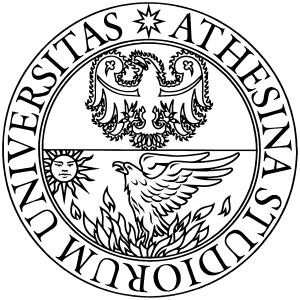
\includegraphics[width=50mm]{logo_bn.png}}
}
\author{Martino Papa}
\date{Day Month Year}

\begin{document}
\maketitle
\tableofcontents

Al momento il documento potrebbe contenere anche definizioni o teoremi “di troppo”. Ho scritto tutto ciò che mi sembrava utile al fine di apprendere fino in fondo l'argomento.

%prerequisiti
\section{Teoria dei grafi}
\begin{definizione}[Grafo]
    Un grafo è una coppia \(G=(V,E)\) dove:
    \begin{itemize}
        \item \(V\) è un insieme di vertici (\textbf{vertex});
        \item \(E\) è un insieme di coppie di nodi \((u,v),\;u,v\in V\) dette archi o lati (\textbf{edge});
    \end{itemize}
    Nei grafi \textbf{orientati} le coppie in \(E\) sono ordinate in quelli non orientati no.
\end{definizione}

\begin{definizione}[Adiacenza]
    Un vertice \(v\) si dice adiacente a \(u\) se esiste \((u,v) \in E\). \\
    NB:\@ nei grafi non orientati l'adiacenza è una relazione simmetrica.
\end{definizione}

\begin{definizione}[Incidente]
    Un arco \((u,v)\) si dice incidente da \(u\) a \(v\).
\end{definizione}

\begin{definizione}[Grado]
    Nel caso di grafi orientati definiamo:
    \begin{itemize}
        \item \textbf{grado entrante} di un nodo come il numero di archi incidenti su esso;
        \item \textbf{grado uscente} di un nodo come il numero di archi incidenti da esso.
    \end{itemize}
    Per i grafi non orientati avremo invece un'unica definizione:
    \begin{itemize}
        \item il \textbf{grado} di un nodo è il numero di archi incidenti su di esso.
    \end{itemize}
\end{definizione}

\begin{definizione}[Cammino]
    Sia \(G=(V,E)\) un grafo. Un cammino \(C\) di lunghezza \(k\) è una sequenza di nodi \(u_0,u_1 \dots, u_k\) t.c.
    \begin{equation}
        (u_i,u_{i+1})\in E \text{ per } 0 \leq i \leq k-1
    \end{equation}
\end{definizione}

\begin{definizione}[Grafi isomorfi]
    Siano \(G=(V(G),E(G)), H=(V(H),E(H))\) due grafi. Diremo \(G\) isomorfo a \(H\) se \(\exists \theta : V(G) \to V(H)\) t.c. \(\theta\) è un isomorfismo e
    \begin{equation}
        \theta(E(G)) \doteq \{ \theta(uv) \; t.c.\; uv \in E(G)\} = E(H)
    \end{equation}
\end{definizione}

\begin{definizione}[Grafo completo]
    Un grafo \(G=(V,E)\) si dice completo se
    \begin{equation}
        \forall u,v \in V \; \exists (u,v) \in E
    \end{equation}
    Definiamo \(K_n\) un grafo completo con \(n\) vertici.
\end{definizione}

\begin{definizione}[Grafo bipartito]
    Un grafo non orientato \(G=(V,E)\) si dice bipartito se \(V\) può essere diviso in due sottoinsiemi \(X,Y\) t.c.
    \begin{equation}
        \forall (u,v) \in E \text{ vale } u\in X,\; v\in Y \text{ oppure } u\in Y,\; v\in X
    \end{equation}
    Un grafo bipartito può avere al più \(|X|\cdot |Y|\) archi. \\
    Definaiamo inoltre \(K_{m,n}\) il grafo bipartito completo che soddisfa
    \begin{equation}
        |X|=m,\; |Y|=n,\; \varepsilon \doteq |E| = mn
    \end{equation}
\end{definizione}

\begin{definizione}[Connessione]
    Un grafo non orientato \(G=(V,E)\) è detto \textbf{connesso} se
    \begin{equation}
        \forall u,v \in V \; \exists (u,v) \in E
    \end{equation}
    Un sottografo connesso massimale di un grafo non orientato è detto \textbf{componente connessa}.
\end{definizione}

\begin{definizione}[Vertex-connectivity]
    Sia \(G=(V,E)\) un grafo non orientato. Definiamo \textbf{vertex-connectivity}  \(\kappa\) il minimo numero di vertici da eliminare per sconnettere \(G\).
\end{definizione}

\begin{definizione}[Grafo k-connesso]
    Sia \(G=(V,E)\) un grafo non orientato. Diremo \(G\) \textbf{k-connesso} se \(|V|>k\) e \(\kappa \geq k\) dove \(\kappa\) corrisponde alla vertex-connectivity.\\
    Informalmente un grafo è detto k-connesso se rimane connesso rimuovendo \(k'<k\) vertici qualsiasi.
\end{definizione}

\begin{teorema}[Grafo 2-connesso]
    Un grafo non orientato \(G=(V,E),\; |V| \geq 3\) è 2-connesso \(\Leftrightarrow\) ogni coppia di vertici \((u,v)\) è connessa da almeno 2 cammini internamente disgiunti.
\end{teorema}

\begin{definizione}[Cammini internamente disgiunti]
    Sia \(G=(V,E)\) un grafo non orientato, siano \(a,b \in V\) due cammini da \(a\) a \(b\) \(a,v_1,\dots,v_n,b\), \(a,u_1,\dots,u_n,b\). Essi si dicono internamente disgiunti se
    \begin{equation}
        v_i \neq u_j\; \forall i,j
    \end{equation}
\end{definizione}

\begin{definizione}[Ciclo di Hamilton]
    Sia \(G=(V,E)\) un grafo non orientato. Definiamo ciclo di Hamilton un ciclo che contiene tutti i vertici del grafo una sola volta.\\
    Definiamo \(G\) hamiltoniano se \(G\) contiene un ciclo di hamilton.
\end{definizione}
% teo

\begin{definizione}[Suddivisione]
    Dato un grafo \(G\) definiamo suddivisione (subdivision) di \(G\) i grafi ottenuti da \(G\) rimpiazzando uno o più archi con cammini di lunghezza 2 o più. In altre parole una suddivisione di \(G\) è un grafo ottenuto da esso inserendo dei vertici “all'interno dei lati”.
\end{definizione}
\begin{figure}[H]
    \centering
    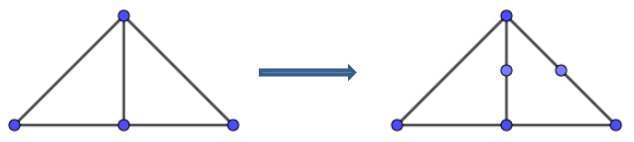
\includegraphics[scale=0.6]{img/suddivisione.PNG}
    \caption{esempio suddivisione}
\end{figure}
\begin{definizione}[Contrazione]
    Operazione inversa della suddivisione, consiste nell'contrarre un arco avente un endpoint di grado 2.
\end{definizione}

\begin{definizione}[Grafi omeomorfi]
    Due grafi \(G_1,G_2\) si dicono topologicamente equivalenti o omeomorfi se possono essere trasformati l'uno nell'altro attraverso operazioni di suddivisione o contrazione degli archi.
    \\ Denotiamo l'insieme dei grafi omeomorfi a \(G\) con \(TG\).
\end{definizione}

\begin{definizione}[Minore]
    Sia \(H\) un grafo ottenuto da \(G\) tramite una sequenza di operazioni di rimozione di archi o vertici o contrazione di archi. \(H\) è detto minore di \(G\).
\end{definizione}

\begin{definizione}[Facial walk]
    Sia \(G\) grafo, \(G^\psi\) una sua immersione nel piano. Un cammino chiuso \(C\) frontiera di una faccia \(F\) di \(G^\psi\) è detto facial walk di F.
\end{definizione}

\begin{definizione}[Grado di una faccia]
    Definaiamo \(\deg(F)\) grado di una faccia \(F\) come la lunghezza del suo facial walk.
\end{definizione}


\section{Topologia}

\begin{definizione}[n-cella chiusa]
    Spazio topologico omeomorfo ad una palla chiusa n-dimensionale.
\end{definizione}
\begin{definizione}[Complesso cellulare (CW-complesso)]
    Spazio topologico ottenuto incollando tra loro un insieme di celle chiuse.
\end{definizione}
\begin{definizione}[Caratteristica di eulero]
    Sia \(\tau \subset \mathbb{R}^n\) un complesso cellulare composto da \(k_i\) i-celle \(i=0,\dots,n\). Definiamo caratteristica di eulero
    \begin{equation}
        \chi(\tau) = k_0 - k_1 + k_2 - \dots k_n = \sum_{i=0}^{n}{(-1)}^i k_i
    \end{equation}
\end{definizione}

\begin{definizione}[Cammini omotopi]
    Siano \(f,g \in \mathcal{C}^0(X;Y)\). Diciamo \(f\) e \(g\) omotope \(f \sim g\) se esiste \(H : X \times [0,1] \to Y\) t.c.
    \begin{equation}
        \forall x \in X \begin{cases}
            H(x,0)=f(x) \\
            H(x,1)=g(x)
        \end{cases}
    \end{equation}
    Informalmente questo vale se una mappa può essere “deformata con continutià” nell'altra.
\end{definizione}

\begin{definizione}[Spazi omotopicamente equivalenti]
    \(X,Y\) si dicono omotopicamente equivalenti (\(X\sim Y\)) se \(\exists f : X \to Y, g:Y \to X \) t.c.
    \begin{itemize}
        \item \(g \circ f \sim id_X\)
        \item \(f \circ g \sim id_Y\)
    \end{itemize}
    Informalmente \(X,Y\) saraano omotopicamente equivalenti se possono essere trasformati l'uno nell'altro con operazioni di deformazione.
\end{definizione}

\begin{lemma}[Omotopicamente invariante]\label{om-inv}
    La caratteristica di eulero è un omotopicamente invariante, ovvero
    \begin{equation}
        X \sim Y \Rightarrow \chi (X) = \chi (Y)
    \end{equation}
\end{lemma}

\begin{proposizione}[Invarianza topologica]\label{inv-top}
    La caratteristica di eulero è un invariante topologico, ovvero
    \begin{equation}
        X \simeq Y \Rightarrow \chi (X) = \chi (Y)
    \end{equation}
    diciamo che \(X \simeq Y\) se \(X\) e \(Y\) sono omeomorfi.
\end{proposizione}

\begin{lemma}
    Ogni poliedro semplice può essere identificato come un grafo planare usando i vertici del poliedro come vertici del grafo e gli spigoli del poliedro come archi del grafo.
\end{lemma}
\begin{proposizione}
    Sia \(\tau\) un poliedro semplice allora \(\chi(\tau)=2\)
    \begin{proof}
        Questo risultato segue direttamente dal lemma precedente e dal teorema \(\ref{formulaeulero}\).
    \end{proof}
\end{proposizione}

\section{Grafi planari}

\begin{definizione}[Grafo planare]
    Un grafo non orientato \(G\) si dice planare se può essere rappresentato nel piano evitando che gli archi si intersechino (se non negli endpoint).
\end{definizione}

\begin{teorema}\label{eulero-generica}
    Sia \(G\) un grafo planare avente \(k\) componenti connesse. Sia \(G^\varphi\) una immersione di \(G\) nel piano, allora
    \begin{equation}
        \chi(G)=V+f-\epsilon = k+1
    \end{equation}
    dove \(V\) è il numero di vertici (\(k_0\)), \(\epsilon\) il numero di archi (\(k_1\)) e \(f\) il numero di facce (\(k_2\)).
    \begin{proof}
        Procediamo per induzione sul numero di archi \( \epsilon \): \smallskip \\
        \underline{caso base \(\epsilon=0\)}, \(V=k\) vertici, \(f=1\) quindi è soddisfatta \(V-\epsilon+f = k+1\)\smallskip \\
        \underline{passo induttivo \(\epsilon \to \epsilon + 1\)}, aggiungiamo un arco al grafo
        \begin{enumerate}
            \item \textit{il nuovo arco è un loop}, in questo caso \(V \to V\), \(\epsilon \to \epsilon +1\), \(f \to f+1\), \(k \to k\) e quindi
                  \begin{equation}
                      V-(\epsilon+1)+(f+1)=V-\epsilon+f=k+1
                  \end{equation}
            \item \textit{il nuovo arco è tra due vertici appartenenti alla stessa componente connessa}, anche in questo caso \(V \to V\), \(\epsilon \to \epsilon +1\), \(f \to f+1\), \(k \to k\) e quindi
                  \begin{equation}
                      V-(\epsilon+1)+(f+1)=V-\epsilon+f=k+1
                  \end{equation}
            \item \textit{il nuovo arco connette due componenti che erano sconnesse}, in questo caso \(V \to V\), \(\epsilon \to \epsilon +1\), \(f \to f\), \(k \to k-1\) e quindi
                  \begin{equation}
                      V-(\epsilon +1)+f = (k-1) + 1 = k'+1
                  \end{equation}
                  dove \(k'=k-1\) è il numero di componenti connesse dopo l'aggiunta dell'arco.
        \end{enumerate}
    \end{proof}
\end{teorema}

\begin{corollario}[Formula di Eulero]\label{formulaeulero}
    Sia \(G\) un grafo planare connesso, allora
    \begin{equation}
        \chi(G)=V+f-\epsilon = 2
    \end{equation}
    \begin{proof}
        Direttamente dal teorema \(\ref{eulero-generica}\) con \(k=1\).
    \end{proof}
\end{corollario}

\begin{proposizione}
    Ogni suddivisione di un grafo non planare è non planare, questo implica anche che i vertici di grado 2 non influenzano la planarità del grafo.
    \begin{proof}
        Sia \(G\) grafo non planare, \(a,b\) due archi che si intersecano nell'immersione \(G^\varphi\), è evidente che suddividere \(a\) o \(b\) non andrebbe ad influire sulla non planarità del grafo.
    \end{proof}
\end{proposizione}

\begin{lemma}\label{gradifacce}
    Sia \(G\) un grafo planare, \(G^\psi\) una sua immersione nel piano, \(F_1, \dots, F_f\) le facce di \(G^\psi\) allora
    \begin{equation}
        \sum_{i=1}^f \deg(F_i) = 2\epsilon
    \end{equation}
    \begin{proof}
        Segue direttamente dal fatto che ogni arco \((u,v)\) è incedente esattamente su due facce di \(G^\psi\).
    \end{proof}
\end{lemma}

\begin{proposizione}\label{criterioNonPlan}
    Sia \(G\) planare, \(\epsilon\) il numero di archi, \(V\) il numero di vertici. Vale allora
    \begin{equation}
        \epsilon \leq 3V - 3
    \end{equation}
    Inoltre se supponiamo \(V \geq 3\) vale
    \begin{equation}
        \epsilon \leq 3V - 6
    \end{equation}
    \begin{proof}
        Sia \(V<3\). In questo caso il lemma è una diretta conseguenza della formula di Eulero (Teorema {\ref{formulaeulero}}). \\
        Sia \(V\geq 3\). \(G\) planare \(\Rightarrow\) ogni faccia ha almeno 3 lati ovvero \(\deg(F_i) \geq 3\; \forall i\). Per il lemma {\ref{gradifacce}} vale quindi
        \begin{equation}
            2\epsilon = \sum_{i=1}^f \deg(F_i) \geq \sum_{i=1}^f 3 = 3f
        \end{equation}
        Per la formula di eulero segue inoltre \(V+f-\epsilon = 2\) da cui abbiamo, moltiplicando per 3 e riarrangiando i termini
        \begin{equation}
            3\epsilon = 3V + 3f - 6
        \end{equation}
        applicando ora \(3f\leq 2 \epsilon\) otteniamo la tesi.
    \end{proof}
\end{proposizione}

\begin{lemma}
    \(K_5\) e \(K_{3,3}\) sono grafi non planari.
    \begin{proof}
        \underline{\(K_5\)}: il grafo completo \(K_n\) ha \(\epsilon=\frac{n(n-1)}{2}\) archi. Supponendo per assurdo \(K_5\) planare dovrebbe valere la proposizione \(\ref{criterioNonPlan}\) ovvero, essendo \(V=5 \geq 3\)
        \begin{equation}
            10 = \frac{n(n-1)}{2} = \epsilon \leq 3V-6 = 9 \rightarrow \text{\Lightning}
        \end{equation}
        \underline{\(K_{3,3}\)}: Supponendo per assurdo \(K_{3,3}\) planare, sapendo \(\epsilon=3*3=9\), \(V=6\) dalla formula di eulero \(\ref{formulaeulero}\) otterremmo \(f=2-V+\epsilon=5\). Siccome \(K_{3,3}\) è bipartito non contiene cicli composti da 3 archi \(\rightarrow\) ogni faccia ha almeno 4 lati, ovvero \(\deg(F)\geq 4 \;\forall F\) vale \(\sum_{i=1}^{f} \deg(F_i) \geq 4*f = 20\). Per il lemma \(\ref{gradifacce}\) dovrebbe valere però
        \begin{equation}
            20 \leq \sum_{i=1}^{f} \deg(F_i) = 2\epsilon = 18 \rightarrow\text{\Lightning}
        \end{equation} 
    \end{proof}
    \begin{figure}[H]
        \centering
        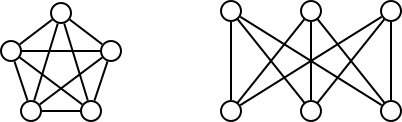
\includegraphics[scale=0.6]{img/k533.PNG}
        \caption{immersione nel piano di \(K_5\) e \(K_{3,3}\)}
    \end{figure} 
\end{lemma}

% metto immagini di K33 K5
\begin{teorema}[Teorema di Kuratowski]
    Un grafo \(G\) è planare se e solo se non contiene sottografi \(TK_{3,3}\) o \(TK_5\).
    \begin{proof}
        \underline{“\(\Rightarrow\)”}: è evidente che se un grafo \(G\) è planare non contiene sottografi omeomorfi a \(K_{3,3}\) o \(K_5\). \smallskip \\
        \underline{“\(\Leftarrow\)”}: per provare questo lato dell'implicazione dimostramo la tesi equivalente “\(G\) non planare \(\Rightarrow\) contiene \(TK_{3,3}\) o \(TK_5\)”
    \end{proof}
\end{teorema}
\noindent Si può riformulare il teorema precedente in termine di minori.
\begin{teorema}[Teorema di Wagner]
    Un grafo \(G\) è planare se e solo se non ha \(K_{3,3}\) o \(K_5\) come minori.
\end{teorema}




% migiorare \ref{}

% LIBRO: graph algorithm and optimization

% Boyer and Myrvold
% triangolazione = massimale?
% grado di un nodo
% come triangolo un grafo planare?
% grafo duale
% sfera <--> piano
% tazza <--> toro
% problema: G è hamiltoniano?
% alleggerimento delle ipotesi ciclo di hamilton 
% non si perde generalità partendo con un grafo 2-connesso
% volendo c'è l'algoritmo per l'inserimento nel piano proiettivo
% grafo non diretto (non si perde generalità testando la planarità)


% is planare?
% stampare K5 o K33 in caso di non planarità
% path addition method (libro) O(n)
% dimostrazione teorema kuratowski
% disegnare i grafi planari quando possibile (?)
% parlare delle possibili applicazioni dei grafi planari
% 


% disegno con linee rette

% algoritmo di dijkstra più efficente per grafi planari
\end{document}